% Options for packages loaded elsewhere
\PassOptionsToPackage{unicode}{hyperref}
\PassOptionsToPackage{hyphens}{url}
\PassOptionsToPackage{dvipsnames,svgnames,x11names}{xcolor}
%
\documentclass[
  letterpaper,
  DIV=11,
  numbers=noendperiod]{scrreprt}

\usepackage{amsmath,amssymb}
\usepackage{iftex}
\ifPDFTeX
  \usepackage[T1]{fontenc}
  \usepackage[utf8]{inputenc}
  \usepackage{textcomp} % provide euro and other symbols
\else % if luatex or xetex
  \usepackage{unicode-math}
  \defaultfontfeatures{Scale=MatchLowercase}
  \defaultfontfeatures[\rmfamily]{Ligatures=TeX,Scale=1}
\fi
\usepackage{lmodern}
\ifPDFTeX\else  
    % xetex/luatex font selection
\fi
% Use upquote if available, for straight quotes in verbatim environments
\IfFileExists{upquote.sty}{\usepackage{upquote}}{}
\IfFileExists{microtype.sty}{% use microtype if available
  \usepackage[]{microtype}
  \UseMicrotypeSet[protrusion]{basicmath} % disable protrusion for tt fonts
}{}
\makeatletter
\@ifundefined{KOMAClassName}{% if non-KOMA class
  \IfFileExists{parskip.sty}{%
    \usepackage{parskip}
  }{% else
    \setlength{\parindent}{0pt}
    \setlength{\parskip}{6pt plus 2pt minus 1pt}}
}{% if KOMA class
  \KOMAoptions{parskip=half}}
\makeatother
\usepackage{xcolor}
\setlength{\emergencystretch}{3em} % prevent overfull lines
\setcounter{secnumdepth}{5}
% Make \paragraph and \subparagraph free-standing
\ifx\paragraph\undefined\else
  \let\oldparagraph\paragraph
  \renewcommand{\paragraph}[1]{\oldparagraph{#1}\mbox{}}
\fi
\ifx\subparagraph\undefined\else
  \let\oldsubparagraph\subparagraph
  \renewcommand{\subparagraph}[1]{\oldsubparagraph{#1}\mbox{}}
\fi

\usepackage{color}
\usepackage{fancyvrb}
\newcommand{\VerbBar}{|}
\newcommand{\VERB}{\Verb[commandchars=\\\{\}]}
\DefineVerbatimEnvironment{Highlighting}{Verbatim}{commandchars=\\\{\}}
% Add ',fontsize=\small' for more characters per line
\usepackage{framed}
\definecolor{shadecolor}{RGB}{241,243,245}
\newenvironment{Shaded}{\begin{snugshade}}{\end{snugshade}}
\newcommand{\AlertTok}[1]{\textcolor[rgb]{0.68,0.00,0.00}{#1}}
\newcommand{\AnnotationTok}[1]{\textcolor[rgb]{0.37,0.37,0.37}{#1}}
\newcommand{\AttributeTok}[1]{\textcolor[rgb]{0.40,0.45,0.13}{#1}}
\newcommand{\BaseNTok}[1]{\textcolor[rgb]{0.68,0.00,0.00}{#1}}
\newcommand{\BuiltInTok}[1]{\textcolor[rgb]{0.00,0.23,0.31}{#1}}
\newcommand{\CharTok}[1]{\textcolor[rgb]{0.13,0.47,0.30}{#1}}
\newcommand{\CommentTok}[1]{\textcolor[rgb]{0.37,0.37,0.37}{#1}}
\newcommand{\CommentVarTok}[1]{\textcolor[rgb]{0.37,0.37,0.37}{\textit{#1}}}
\newcommand{\ConstantTok}[1]{\textcolor[rgb]{0.56,0.35,0.01}{#1}}
\newcommand{\ControlFlowTok}[1]{\textcolor[rgb]{0.00,0.23,0.31}{#1}}
\newcommand{\DataTypeTok}[1]{\textcolor[rgb]{0.68,0.00,0.00}{#1}}
\newcommand{\DecValTok}[1]{\textcolor[rgb]{0.68,0.00,0.00}{#1}}
\newcommand{\DocumentationTok}[1]{\textcolor[rgb]{0.37,0.37,0.37}{\textit{#1}}}
\newcommand{\ErrorTok}[1]{\textcolor[rgb]{0.68,0.00,0.00}{#1}}
\newcommand{\ExtensionTok}[1]{\textcolor[rgb]{0.00,0.23,0.31}{#1}}
\newcommand{\FloatTok}[1]{\textcolor[rgb]{0.68,0.00,0.00}{#1}}
\newcommand{\FunctionTok}[1]{\textcolor[rgb]{0.28,0.35,0.67}{#1}}
\newcommand{\ImportTok}[1]{\textcolor[rgb]{0.00,0.46,0.62}{#1}}
\newcommand{\InformationTok}[1]{\textcolor[rgb]{0.37,0.37,0.37}{#1}}
\newcommand{\KeywordTok}[1]{\textcolor[rgb]{0.00,0.23,0.31}{#1}}
\newcommand{\NormalTok}[1]{\textcolor[rgb]{0.00,0.23,0.31}{#1}}
\newcommand{\OperatorTok}[1]{\textcolor[rgb]{0.37,0.37,0.37}{#1}}
\newcommand{\OtherTok}[1]{\textcolor[rgb]{0.00,0.23,0.31}{#1}}
\newcommand{\PreprocessorTok}[1]{\textcolor[rgb]{0.68,0.00,0.00}{#1}}
\newcommand{\RegionMarkerTok}[1]{\textcolor[rgb]{0.00,0.23,0.31}{#1}}
\newcommand{\SpecialCharTok}[1]{\textcolor[rgb]{0.37,0.37,0.37}{#1}}
\newcommand{\SpecialStringTok}[1]{\textcolor[rgb]{0.13,0.47,0.30}{#1}}
\newcommand{\StringTok}[1]{\textcolor[rgb]{0.13,0.47,0.30}{#1}}
\newcommand{\VariableTok}[1]{\textcolor[rgb]{0.07,0.07,0.07}{#1}}
\newcommand{\VerbatimStringTok}[1]{\textcolor[rgb]{0.13,0.47,0.30}{#1}}
\newcommand{\WarningTok}[1]{\textcolor[rgb]{0.37,0.37,0.37}{\textit{#1}}}

\providecommand{\tightlist}{%
  \setlength{\itemsep}{0pt}\setlength{\parskip}{0pt}}\usepackage{longtable,booktabs,array}
\usepackage{calc} % for calculating minipage widths
% Correct order of tables after \paragraph or \subparagraph
\usepackage{etoolbox}
\makeatletter
\patchcmd\longtable{\par}{\if@noskipsec\mbox{}\fi\par}{}{}
\makeatother
% Allow footnotes in longtable head/foot
\IfFileExists{footnotehyper.sty}{\usepackage{footnotehyper}}{\usepackage{footnote}}
\makesavenoteenv{longtable}
\usepackage{graphicx}
\makeatletter
\def\maxwidth{\ifdim\Gin@nat@width>\linewidth\linewidth\else\Gin@nat@width\fi}
\def\maxheight{\ifdim\Gin@nat@height>\textheight\textheight\else\Gin@nat@height\fi}
\makeatother
% Scale images if necessary, so that they will not overflow the page
% margins by default, and it is still possible to overwrite the defaults
% using explicit options in \includegraphics[width, height, ...]{}
\setkeys{Gin}{width=\maxwidth,height=\maxheight,keepaspectratio}
% Set default figure placement to htbp
\makeatletter
\def\fps@figure{htbp}
\makeatother
\newlength{\cslhangindent}
\setlength{\cslhangindent}{1.5em}
\newlength{\csllabelwidth}
\setlength{\csllabelwidth}{3em}
\newlength{\cslentryspacingunit} % times entry-spacing
\setlength{\cslentryspacingunit}{\parskip}
\newenvironment{CSLReferences}[2] % #1 hanging-ident, #2 entry spacing
 {% don't indent paragraphs
  \setlength{\parindent}{0pt}
  % turn on hanging indent if param 1 is 1
  \ifodd #1
  \let\oldpar\par
  \def\par{\hangindent=\cslhangindent\oldpar}
  \fi
  % set entry spacing
  \setlength{\parskip}{#2\cslentryspacingunit}
 }%
 {}
\usepackage{calc}
\newcommand{\CSLBlock}[1]{#1\hfill\break}
\newcommand{\CSLLeftMargin}[1]{\parbox[t]{\csllabelwidth}{#1}}
\newcommand{\CSLRightInline}[1]{\parbox[t]{\linewidth - \csllabelwidth}{#1}\break}
\newcommand{\CSLIndent}[1]{\hspace{\cslhangindent}#1}

\KOMAoption{captions}{tableheading}
\makeatletter
\makeatother
\makeatletter
\@ifpackageloaded{bookmark}{}{\usepackage{bookmark}}
\makeatother
\makeatletter
\@ifpackageloaded{caption}{}{\usepackage{caption}}
\AtBeginDocument{%
\ifdefined\contentsname
  \renewcommand*\contentsname{Table of contents}
\else
  \newcommand\contentsname{Table of contents}
\fi
\ifdefined\listfigurename
  \renewcommand*\listfigurename{List of Figures}
\else
  \newcommand\listfigurename{List of Figures}
\fi
\ifdefined\listtablename
  \renewcommand*\listtablename{List of Tables}
\else
  \newcommand\listtablename{List of Tables}
\fi
\ifdefined\figurename
  \renewcommand*\figurename{Figure}
\else
  \newcommand\figurename{Figure}
\fi
\ifdefined\tablename
  \renewcommand*\tablename{Table}
\else
  \newcommand\tablename{Table}
\fi
}
\@ifpackageloaded{float}{}{\usepackage{float}}
\floatstyle{ruled}
\@ifundefined{c@chapter}{\newfloat{codelisting}{h}{lop}}{\newfloat{codelisting}{h}{lop}[chapter]}
\floatname{codelisting}{Listing}
\newcommand*\listoflistings{\listof{codelisting}{List of Listings}}
\makeatother
\makeatletter
\@ifpackageloaded{caption}{}{\usepackage{caption}}
\@ifpackageloaded{subcaption}{}{\usepackage{subcaption}}
\makeatother
\makeatletter
\@ifpackageloaded{tcolorbox}{}{\usepackage[skins,breakable]{tcolorbox}}
\makeatother
\makeatletter
\@ifundefined{shadecolor}{\definecolor{shadecolor}{rgb}{.97, .97, .97}}
\makeatother
\makeatletter
\makeatother
\makeatletter
\makeatother
\ifLuaTeX
  \usepackage{selnolig}  % disable illegal ligatures
\fi
\IfFileExists{bookmark.sty}{\usepackage{bookmark}}{\usepackage{hyperref}}
\IfFileExists{xurl.sty}{\usepackage{xurl}}{} % add URL line breaks if available
\urlstyle{same} % disable monospaced font for URLs
\hypersetup{
  pdftitle={Learning\_diary\_F},
  pdfauthor={Shalom Kobby Ampiaw},
  colorlinks=true,
  linkcolor={blue},
  filecolor={Maroon},
  citecolor={Blue},
  urlcolor={Blue},
  pdfcreator={LaTeX via pandoc}}

\title{Learning\_diary\_F}
\author{Shalom Kobby Ampiaw}
\date{2025-11-03}

\begin{document}
\maketitle
\ifdefined\Shaded\renewenvironment{Shaded}{\begin{tcolorbox}[breakable, borderline west={3pt}{0pt}{shadecolor}, frame hidden, interior hidden, enhanced, sharp corners, boxrule=0pt]}{\end{tcolorbox}}\fi

\renewcommand*\contentsname{Table of contents}
{
\hypersetup{linkcolor=}
\setcounter{tocdepth}{2}
\tableofcontents
}
\bookmarksetup{startatroot}

\hypertarget{preface}{%
\chapter*{Preface}\label{preface}}
\addcontentsline{toc}{chapter}{Preface}

\markboth{Preface}{Preface}

This is a Quarto book.

To learn more about Quarto books visit \#

\begin{Shaded}
\begin{Highlighting}[]
\CommentTok{\#1 + 1}
\end{Highlighting}
\end{Shaded}

\bookmarksetup{startatroot}

\hypertarget{introduction}{%
\chapter{Introduction}\label{introduction}}

This is a book created from markdown and executable code.

See Knuth (1984) for additional discussion of literate programming.

\begin{Shaded}
\begin{Highlighting}[]
\DecValTok{1} \SpecialCharTok{+} \DecValTok{1}
\end{Highlighting}
\end{Shaded}

\begin{verbatim}
[1] 2
\end{verbatim}

\bookmarksetup{startatroot}

\hypertarget{introduction-to-remote-sensing-satellite-data}{%
\chapter{Introduction to Remote Sensing \& Satellite
Data}\label{introduction-to-remote-sensing-satellite-data}}

\hypertarget{introduction-1}{%
\section{Introduction}\label{introduction-1}}

This is the first week of remote sensing module. I will first like to
state a brief overview of what it entails.

\begin{figure}

{\centering 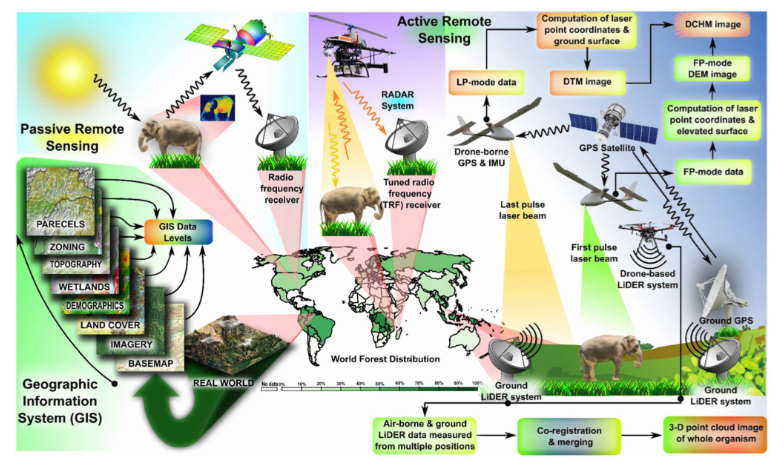
\includegraphics{learning_dairy/week_1/download2.png}

}

\caption{Overview of Remote Sensing}

\end{figure}

Remote sensing for me is a method gathered about the Earth's surface
without direct contact through passive (e.g., satellite imagery) and
active (e.g., LIDAR, RADAR) sensors. It can be integrated with GIS to
analyse landscapes, land cover, demographics and others. Active sensors
compute elevation using laser pulses, while passive sensors capture
reflected sunlight, they all are electromagnetic waves. Combining these
techniques and noting the interaction in the earth's atmosphere, enables
precise environmental monitoring, resource management, and biodiversity
conservation at multiple spatial scales. Satellites I want to delve
deeper into the suspend equipment above the atmosphere - Satellites. I
find it interesting because when I think of remote sensing satellites
come to mind. These satellites are sent up to the earth's orbit. There
are types of satellites. These are

\begin{itemize}
\tightlist
\item
  \textbf{Geostationary Satellites} - These are stationary satellites
  which are normally used for weather monitoring, telecommunications and
  environmental observations.
\item
  \textbf{Low Earth Orbit (LEO) Satellites}: These satellites are used
  for high-resolution imaging has it is normally placed 160 and 2,000 km
  above Earth's surface.
\item
  \textbf{Sun-Synchronous (Polar) Satellites} -- Just like the same,
  these satellites orbit the earth in a polar direction and in sync with
  the sun. This is most used for scientific and environmental
  monitoring.
\end{itemize}

Among these types of satellites, I want to focus on the sun-synchronous
types mainly Sentinel and Landsat satellite. Two main satellites stand
out in remote sensing.

Types of sensors on both types

\begin{longtable}[]{@{}lll@{}}
\toprule\noalign{}
Feature & Landsat-8 & Sentinel-2 \\
\midrule\noalign{}
\endhead
\bottomrule\noalign{}
\endlastfoot
Resolution & 30m & 10-60m \\
Revisit Time & 16days & 5days \\
Bands & 11 bands & 13 bands \\
\end{longtable}

Let's look deeper into the bands Basically, bands are like different
filters with specific wavelengths that satellites use to capture images
of the earth surface. Thus, each band serves a specific purpose and for
what it is best suited for. The USGS comparison graph (USGS, n.d.)
illustrates how different bands on Landsat and Sentinel-2 cover
different portions of the electromagnetic spectrum.

Looking at the image here

\begin{figure}

{\centering 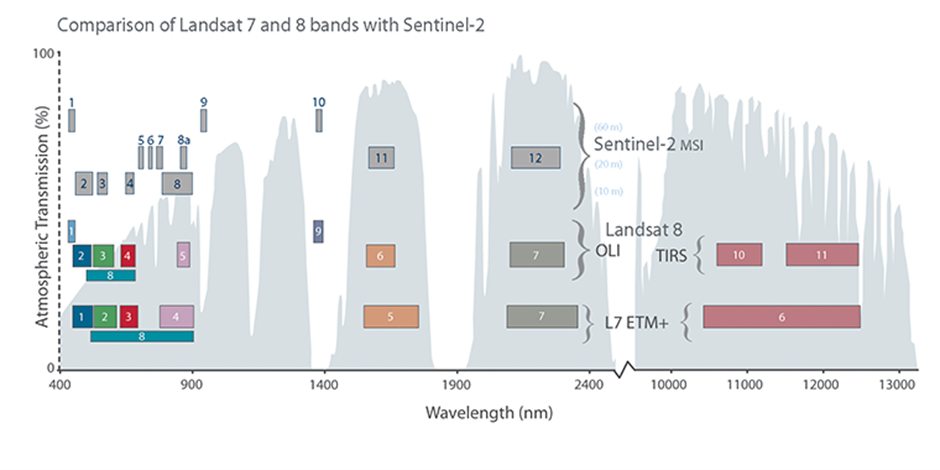
\includegraphics{learning_dairy/week_1/Comparison of Landsat 7 and 8 bands with Sentinel-2.png}

}

\caption{Comparison of Landsat 7 and 8 bands with Sentinel-2}

\end{figure}

In the graph, the x axis presents the wavelength of the electromagnetic
spectrum and y which shows the atmospheric transmission (\%) indicates
the amount of light passing through the atmosphere. The bands are
important for me because I believe they tell a lot about what the data
can be best used for and help in narrowing down which satellite to use
in a study. Here is a summary of the bands and that use case.

\hypertarget{application}{%
\section{Application}\label{application}}

For this section, I want to use what I learnt in summary to understand
which satellite to use for land cover classification. A study by Ahady,
A.B., and Kaplan, G. shows the comparison between Landsat-8 and
Sentinel-2 data over the city of Kabul. This was a comparison over
accuracy of land cover considering water, cropland, urban, and bare
land.

Key insights

The Landsat-8 had an overall classification accuracy 85.04\%. while the
Sentinel-2 had a classification accuracy of 94.26\%. Now lets look at
these images
\includegraphics{learning_dairy/week_1/Landsat-8’s classification.png}

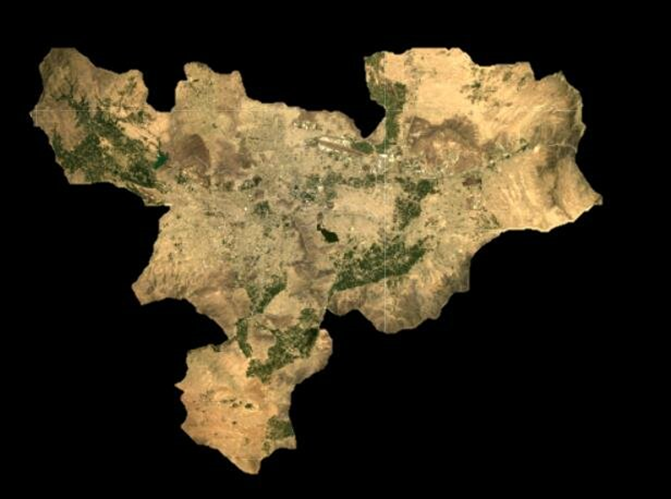
\includegraphics{learning_dairy/week_1/Sentinel-2 classification.png}
From the images we can see that Figure 2 has finer detail as compared to
figure one. This may be due to several reasons, but I feel it's mainly
due to spatial resolution. The sentinel has a higher resolution, so it
expected to have an influence on its accuracy, as it as able to define
features more clearly. Another factor accounting for higher accuracy
maybe the number of visits. The sentinel has shorter revisit period,
thus more volume of data can be gathered in a month as compared to the
Landsat data. Thus, a higher chance of getting an image with little
interference hence a high accuracy. Lastly, I want to check the bands.
This also has major effect on accuracy. As stated earlier, spectral
bands are essential filters that satellites use to analyze Earth's
surface. Ahady \& Kaplan's classification relied on surface reflectance
bands, which directly tie back to the band functions I described in Week
1. The near-infrared (NIR, B5 for Landsat and B8 for Sentinel-2) played
a key role in differentiating urban and vegetative areas, further
demonstrating the importance of understanding band selection in remote
sensing applications.

This does not go to say we can poke holes in the results of the study.
One can be model used in analysing the data. These pictures are cut
clips of the same location and I'm not sure both satellites can capture
the same location within a single tile. So, merging might have been done
hence reducing the robustness of the result. This doesn't go to say
Landsat is better at land cover than sentinel satellite.

\hypertarget{reflection}{%
\section{Reflection}\label{reflection}}

It is the first week of the term and has been a slow start. Still
wondering what I can make out the course and maybe in week 10 will
probably have one. I now understand the bases of the remote sensing,

what are they?

excluding the analysis part. From the summary and application part, I am
wondering if data from both Landsat and Sentinel can use concurrently in
a study. Probable if the data was merged, we will have the wealth of
historical data from the landsat series and the accuracy of the sentinel
data. This can be used in understanding trends of natural disasters or
the climate change\ldots how

. These two do not

\begin{itemize}
\item
  context: how do you think this could used - landcover, pollution
  montiroing (S5P) and why might that be useful
\item
  future exploration
\item
  did you like SNAP, what were limtations of it and
\end{itemize}

Intro to papers

Criticality of papers

\bookmarksetup{startatroot}

\hypertarget{summary}{%
\chapter{Summary}\label{summary}}

In summary, this book has no content whatsoever.

\begin{Shaded}
\begin{Highlighting}[]
\DecValTok{1} \SpecialCharTok{+} \DecValTok{1}
\end{Highlighting}
\end{Shaded}

\begin{verbatim}
[1] 2
\end{verbatim}

\bookmarksetup{startatroot}

\hypertarget{references}{%
\chapter*{References}\label{references}}
\addcontentsline{toc}{chapter}{References}

\markboth{References}{References}

\hypertarget{refs}{}
\begin{CSLReferences}{1}{0}
\leavevmode\vadjust pre{\hypertarget{ref-knuth84}{}}%
Knuth, Donald E. 1984. {``Literate Programming.''} \emph{Comput. J.} 27
(2): 97--111. \url{https://doi.org/10.1093/comjnl/27.2.97}.

\end{CSLReferences}



\end{document}
